\documentclass{beamer}

% for themes, etc.
\mode<presentation>
{ \usetheme{metropolis} }
%{ \usetheme{boxes} }

\usepackage{times}  % fonts are up to you
\usepackage{graphicx}

% these will be used later in the title page
\title{CHPC WLCG Tier2 Facility}
\author{Sean Murray \\
    ALICE \\
    CHPC \\
    CSIR 
}
\date{July 7, 2016}

% note: do NOT include a \maketitle line; also note that this title
% material goes BEFORE the \begin{document}

% have this if you'd like a recurring outline
\AtBeginSection[]  % "Beamer, do the following at the start of every section"
{
\begin{frame}<beamer> 
\frametitle{Outline} % make a frame titled "Outline"
\tableofcontents[currentsection]  % show TOC and highlight current section
\end{frame}
}

\begin{document}

% this prints title, author etc. info from above
\begin{frame}
\titlepage
\end{frame}

\section{WLCG}

\begin{frame}
\frametitle{What is the WLCG}
\centering{
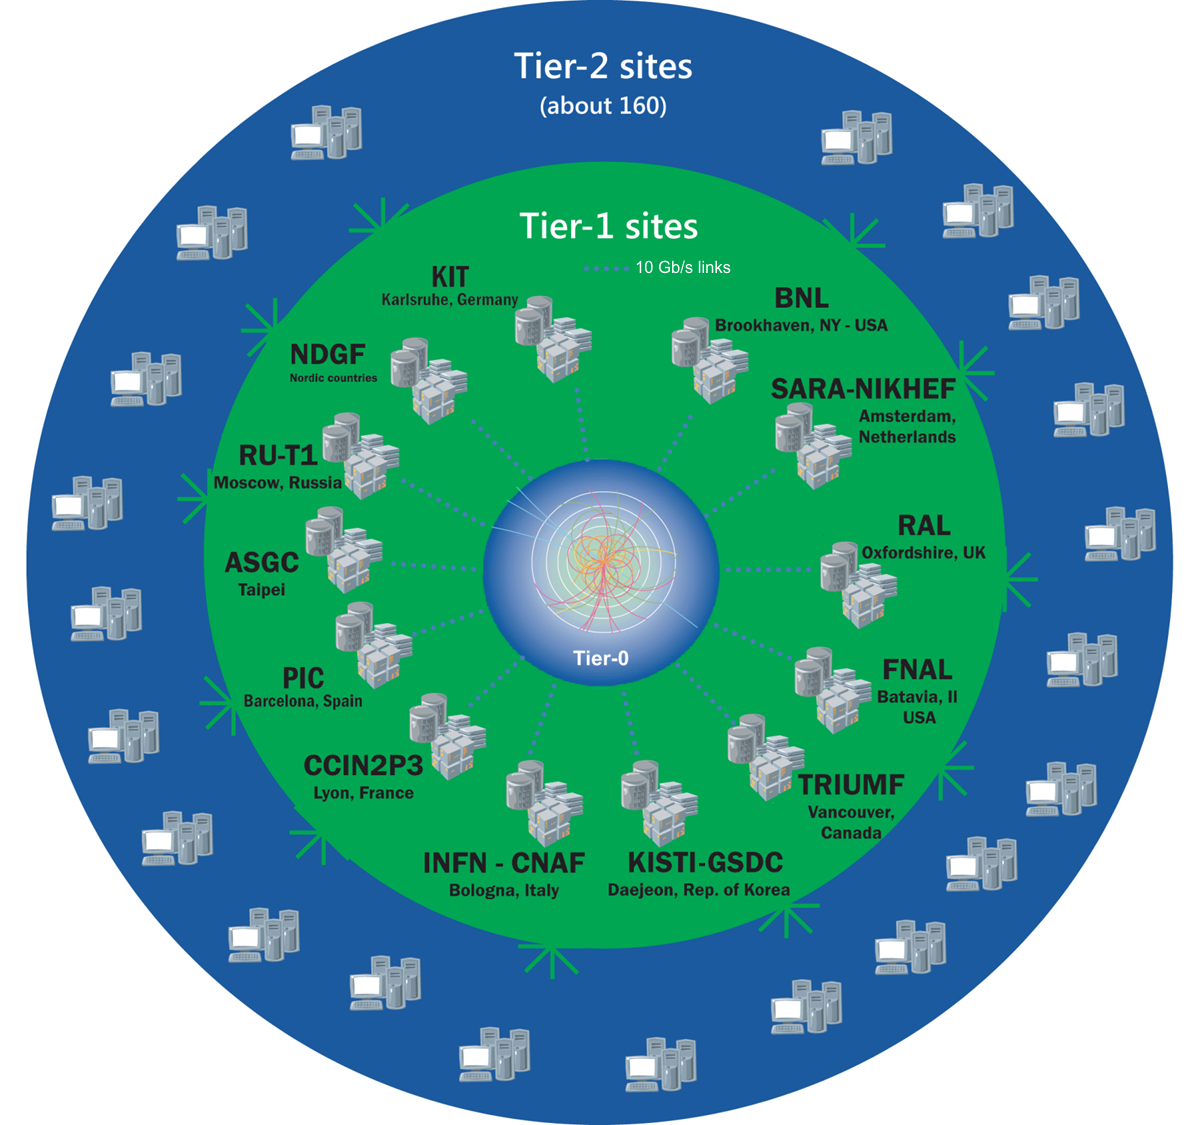
\includegraphics[scale=0.4]{WLCG-TiersJun14_v9.png}
}
\end{frame}
\begin{frame}
\frametitle{WLCG Map of Sites}
\centering{
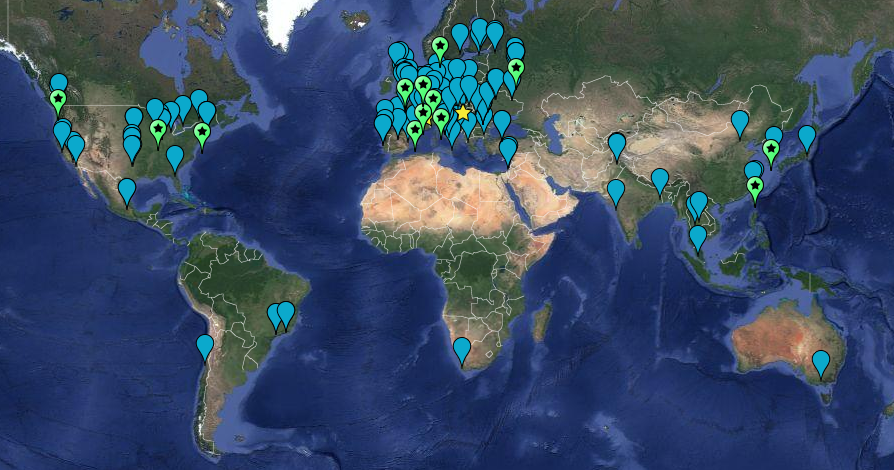
\includegraphics[scale=0.5]{WLCG-Sites.png}
}
\end{frame}

\begin{frame}
\frametitle{WLCG MOU Signed}
\begin{columns}[T] % align columns
\begin{column}{.48\textwidth}
  
\includegraphics[scale=0.45]{CHPCLogo.pdf}
  
\includegraphics[scale=0.45]{WLCGLogo.pdf}
\end{column}%
\begin{column}{.48\textwidth}
  \centering{
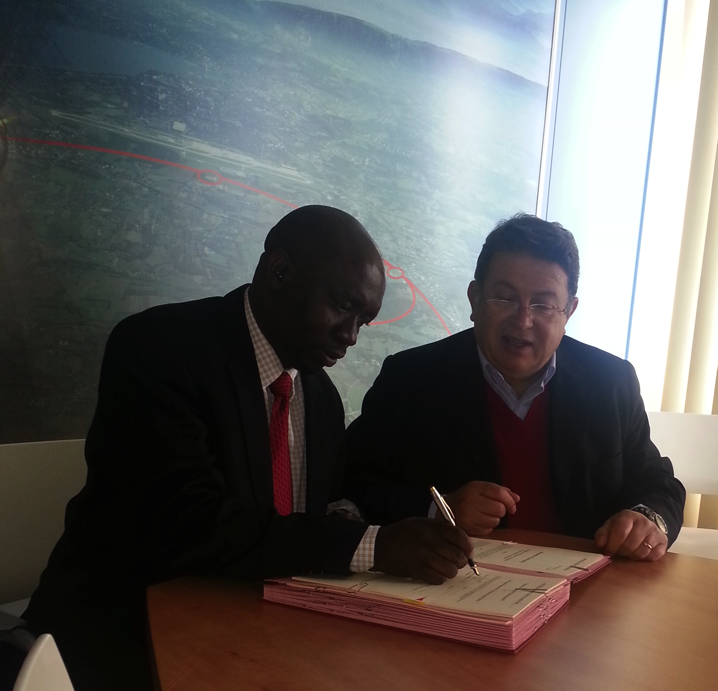
\includegraphics[scale=0.45]{WLCG-MOU_Signing.pdf}
} 
\end{column}%
\end{columns}  
\centering{28 April 2015}
\end{frame}

\begin{frame}
\frametitle{Commitments}
According to Tender :
\begin{itemize}
  \item ALICE 600 cores
  \item ATLAS 600 cores
  \item ALICE 400TB
  \item ATLAS 400TB
\end{itemize}
According to :
https://wlcg-rebus.cern.ch/apps/pledges/resources/
\begin{itemize}
  \item 6000 HEPSPEC06 cores (560 of our cores)
  \item 100TB storage
  \item All ALICE.
\end{itemize}
\end{frame}

\begin{frame}
  \frametitle{Computing Infrastructure}
  \centering{
  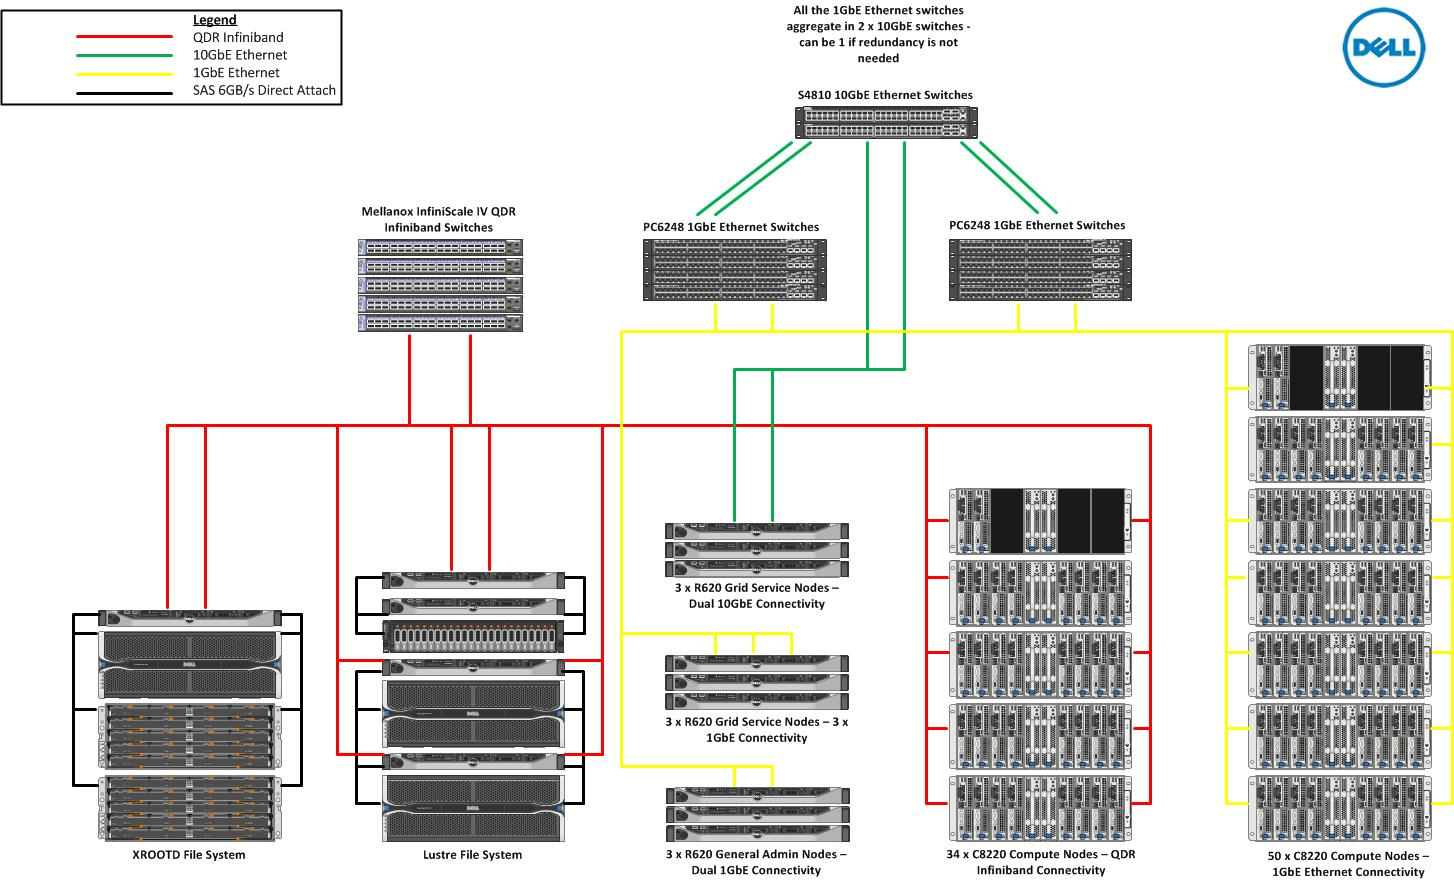
\includegraphics[scale=0.30]{CHPCConnectivityDiagram.jpg}
  }
\end{frame}

\begin{frame}
  \frametitle{Current hardware}
  \begin{itemize}
    \item 50 nodes of 48 cores 192GB RAM and 1.6TB of SSD, 1G ethernet
    \item 34 nodes of 48 cores 96GB RAM and 1TB, FDR infiniband, 6 ``stolen''
    \item 100TB of Lustre on the 34 nodes with FDR infiniband.
    \item 9 management servers, lower spec 
  \begin{itemize}
    \item compute element (head node,ce),
    \item storage element 2 redirectors, 2 storage nodes with direct attached multipath storage
    \item authentication, user interface (gone), monitoring, provisioning. 
  \end{itemize}
  \end{itemize}
\end{frame}

\begin{frame}
  \frametitle{Current Storage}
  \begin{itemize}
    \item 383TB EOS for ALICE, down from 440TB
    \item 252 TB EOS for ATLAS, down from 400TB
    \item 107 TB lustre for 34 nodes.
    \item 104 TB EMC for ATLAS, dead.
  \end{itemize}
\end{frame}


\begin{frame}
  \frametitle{Current Performance}
\begin{itemize}
  \item 465k ALICE jobs in last year
  \item Avg concurrent jobs 704.
  \item ALICE 358TB storage live 17 June
\end{itemize}
\end{frame}

\begin{frame}
  \frametitle{Availability / Reliability}
  So who monitors us :
  \begin{itemize}
    \item WLCG
    \item EGI
    \item ALICE
    \item ATLAS
    \item me via zabbix/grafana and AAROC 
  \end{itemize}

\end{frame}

\begin{frame}
  \frametitle{Grafana ALICE}
  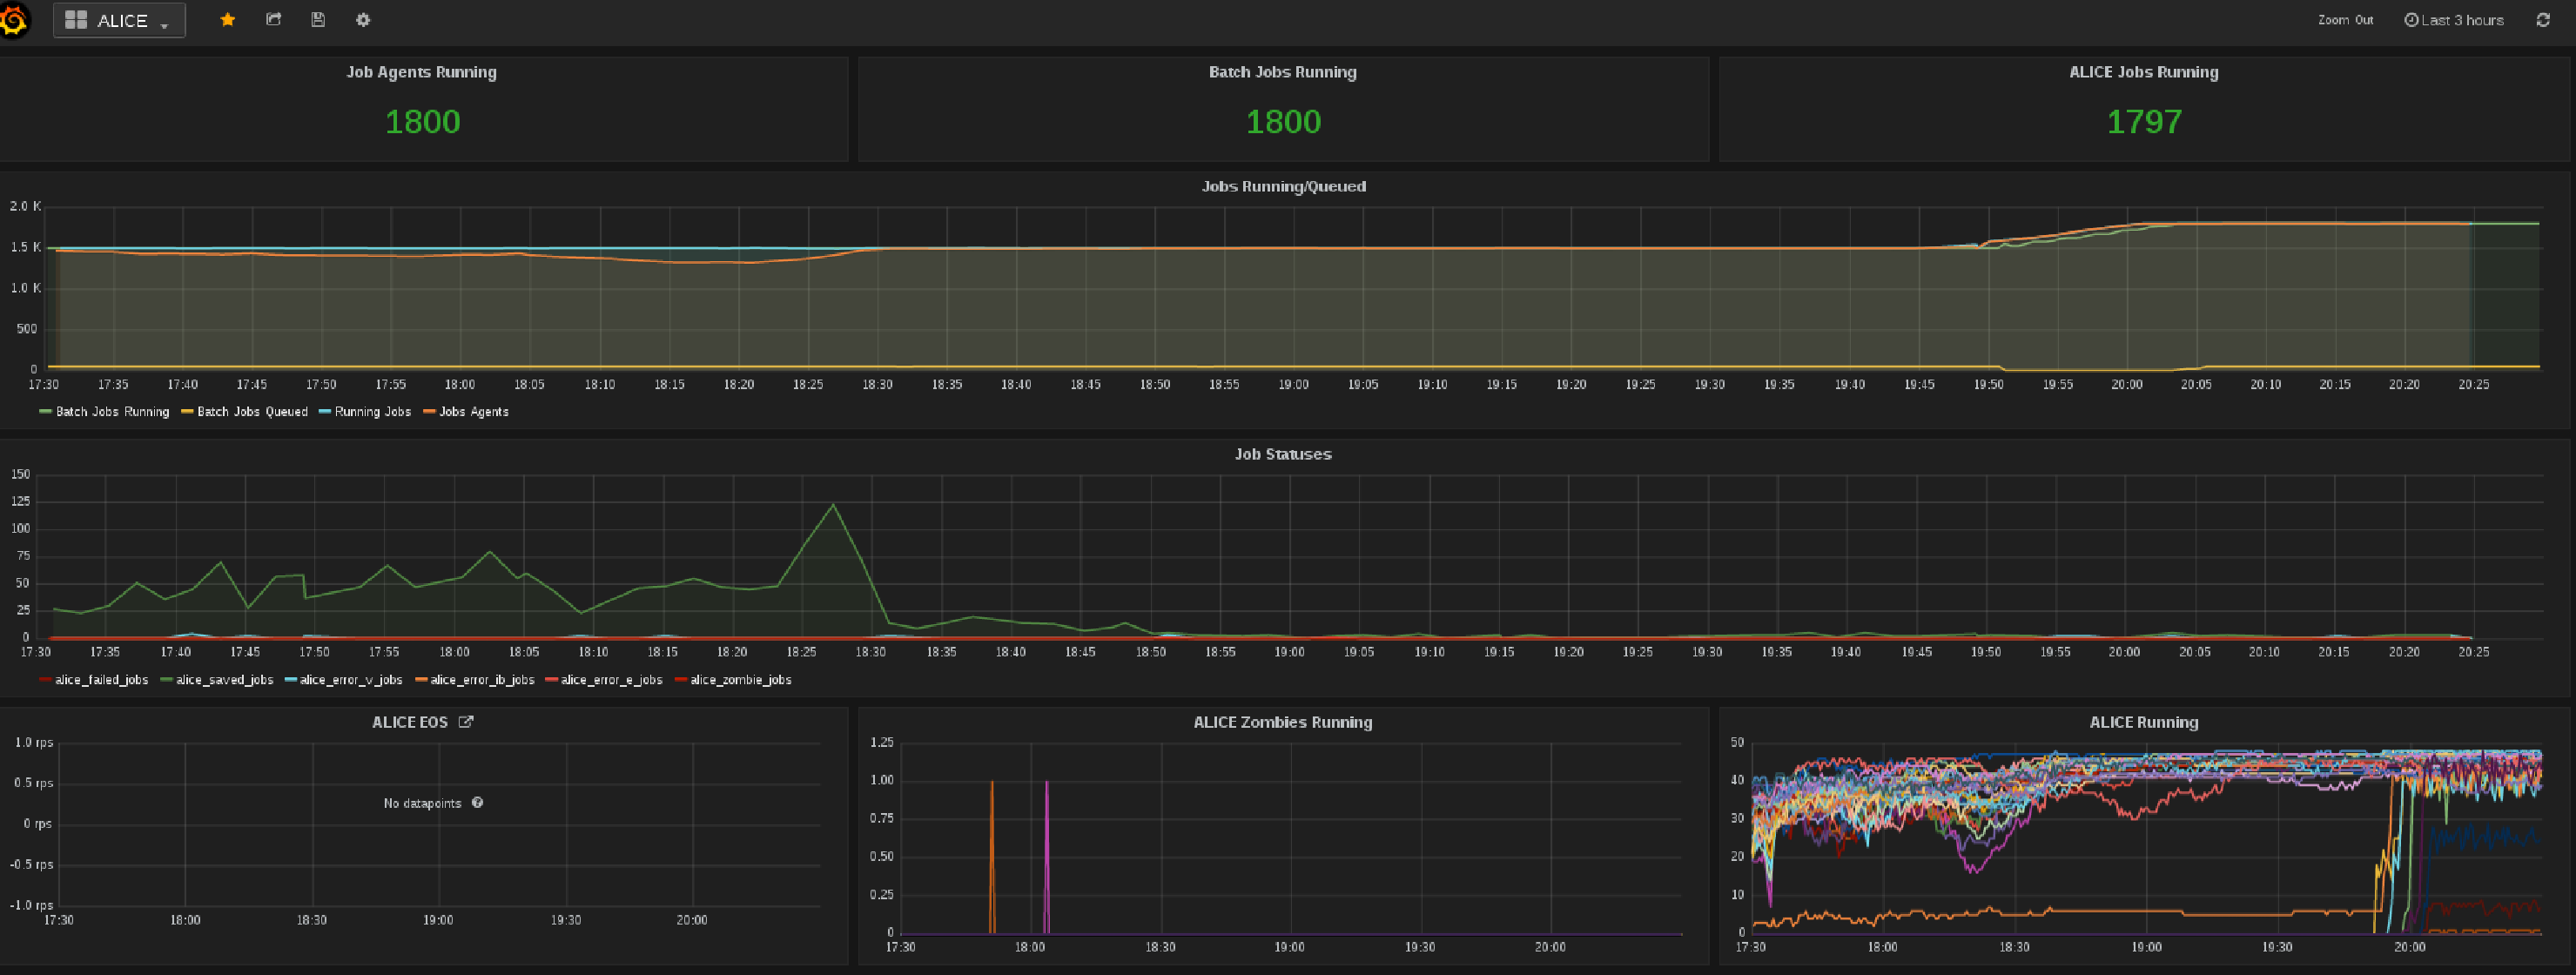
\includegraphics[scale=0.25]{ALICEProcessing-Grafana.pdf}
  This is currently being expanded to pull in more from MonaLisa.
\end{frame}

\begin{frame}
\frametitle{Problems}
It has not been an easy 4 months.
\begin{itemize}
  \item [17 Mar] Switch dies, kills everything, Thursday evening of course, redundancy ?
  \item [14 Apr] disk dies, 15/16 April rebuild fails.
  \item [21May] Site Power upgrade whole weekend.
  \item [22 Jun] General Power failure
\end{itemize}
\end{frame}
\begin{frame}
  \frametitle{Our Data's Scenic Tour}
  \centering{
  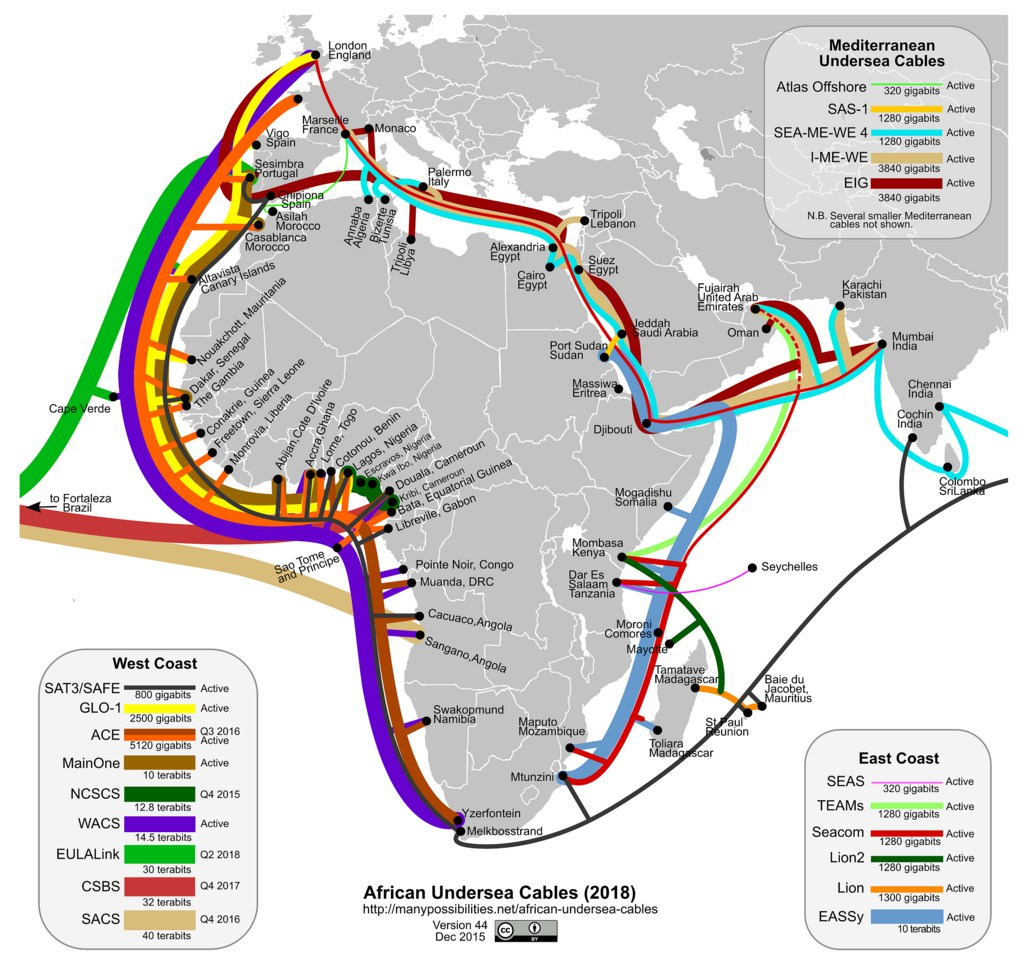
\includegraphics[scale=1]{african_undersea_cables.jpg}
  }
\end{frame}
\begin{frame}
  \frametitle{Data Traffic Mid June}
  \centering{
  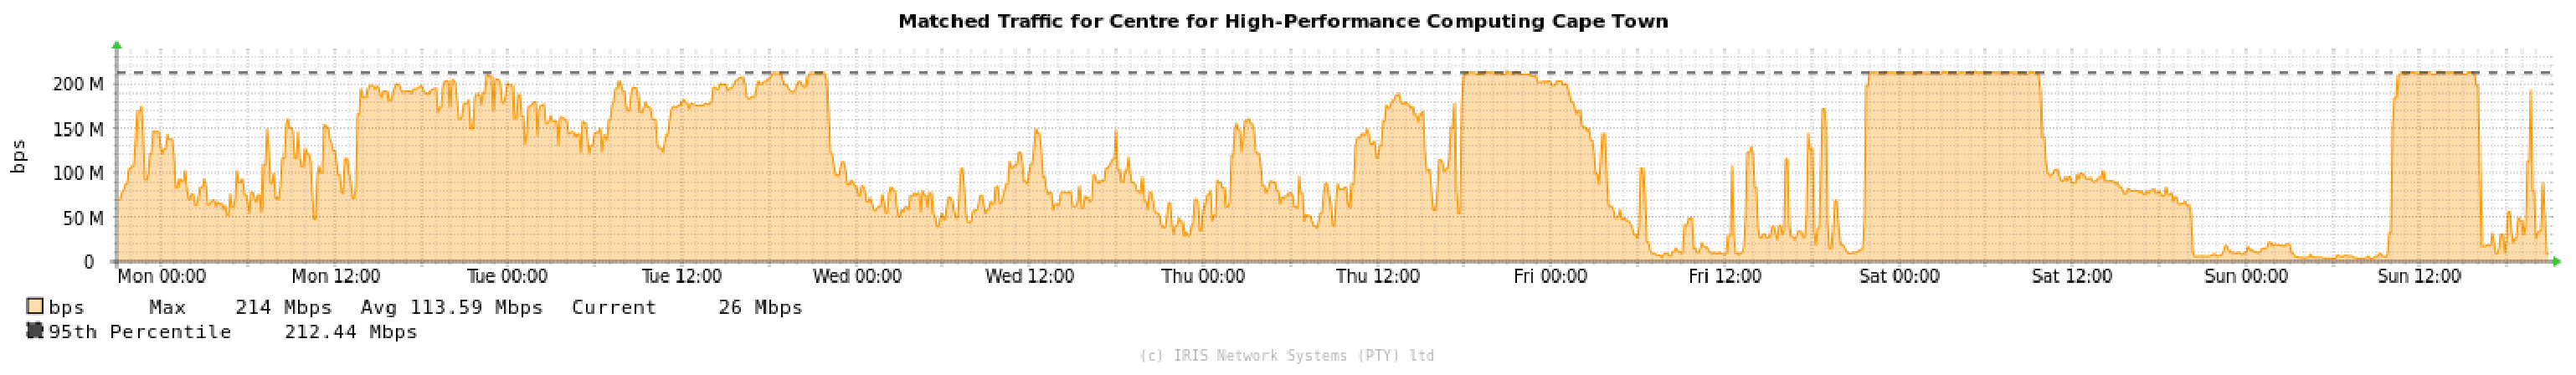
\includegraphics[scale=0.25]{wacsinmidjun.pdf}\\
  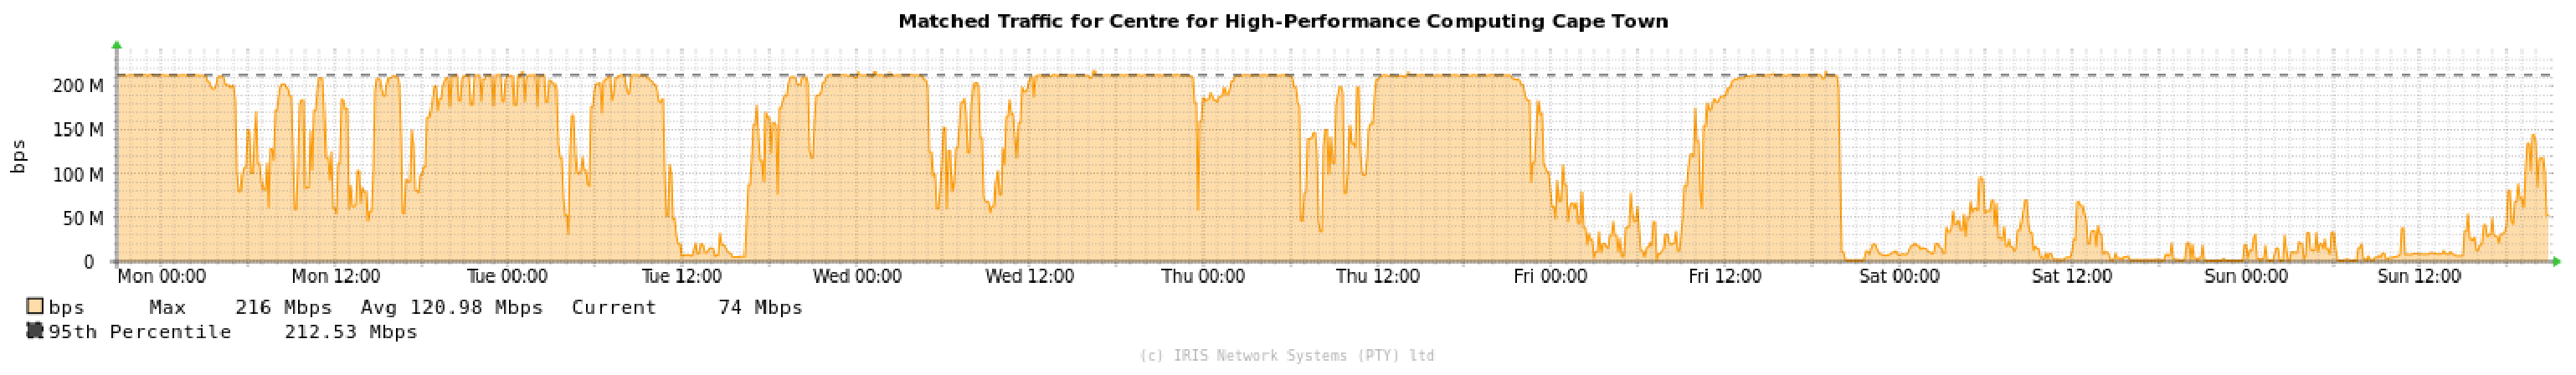
\includegraphics[scale=0.25]{seacomoutmidjun.pdf}
  }
\end{frame}

\begin{frame}
  \frametitle{upgrades}
  \begin{itemize}
    \item attempts to delay till CC7 validation have failed.
    \item Puppify, to auto site deployment, r10k an issue.
    \item Transition to foreman from xcat.
    \item Fix ATLAS Storage (reinstall)
    \item upgrade monitoring server to zabbix3 and new grafana to technical reasons.
    \item Rewire whole network, repower to monitored pdu, and monitor all.
    \item Add inherent redundancy into 10G interfaces on ce,se,se2.
    \item Reinstall while TRYING to keep A/R. problems are vobox and ce. 
    \item Storage, we need an additional 750TB for ALICE and ATLAS.
  \end{itemize}
\end{frame}
\begin{frame}
  \frametitle{Computing Infrastructure}
  \centering{
  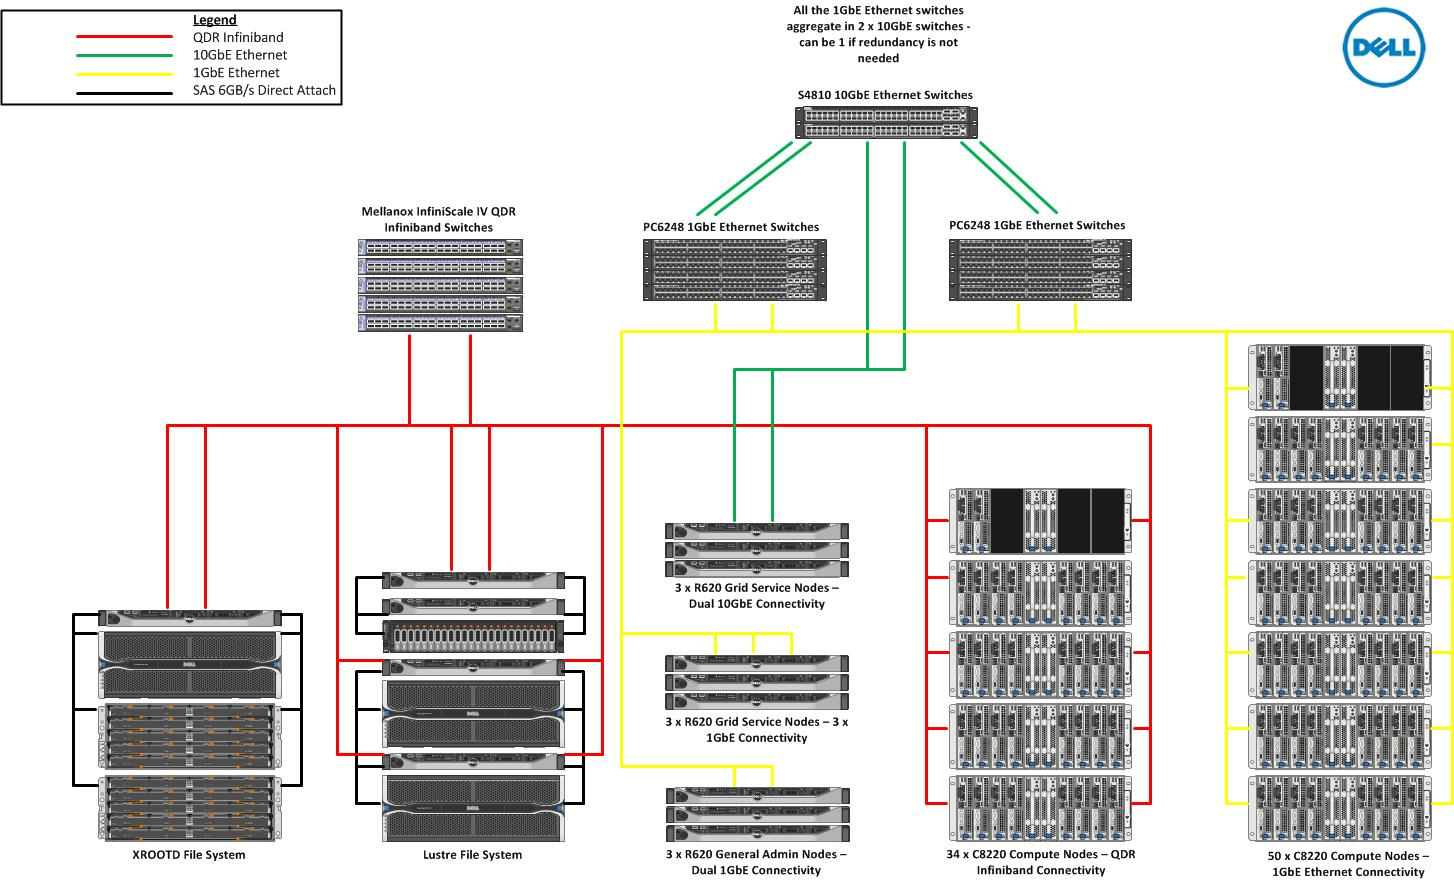
\includegraphics[scale=0.30]{CHPCConnectivityDiagram.jpg}
  }
\end{frame}
\begin{frame}
  \frametitle{Transparency}
  Historically this has not been great, so \ldots
  \begin{itemize}
    \item Federated logins to zabbix and grafana, i.e. You
    \item All code on github in line with AAROC
    \item All issues PUBLIC on github
    \item Still have GGUS for normal tickets.
    \item Some training on the user analysis facility (hopefully online)
    \item A couple of things remain private like network diagrams, obviously, and passwords.
    \item AAROC slac channels.
  \end{itemize}
\end{frame}
\begin{frame}
  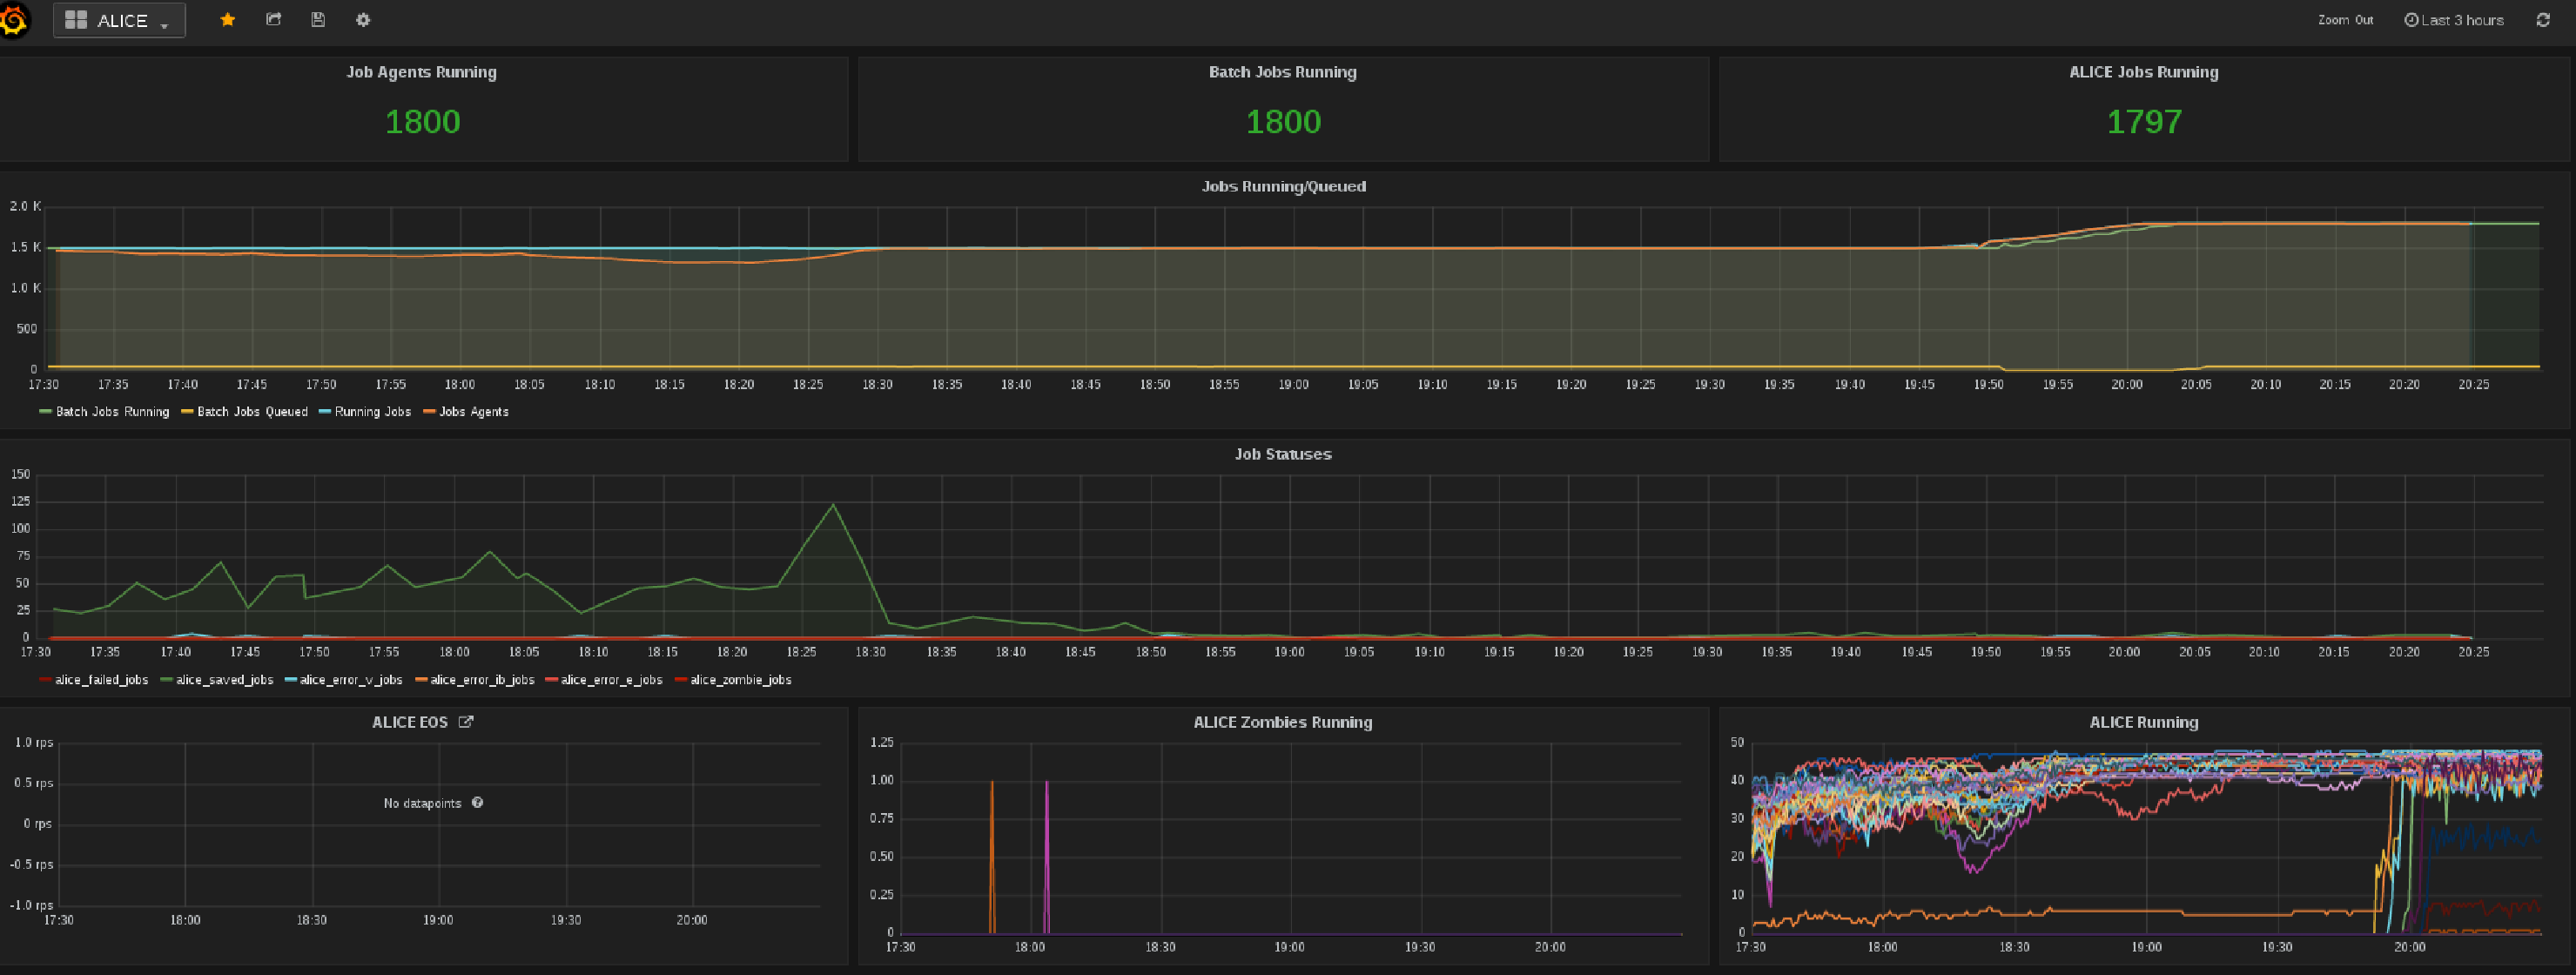
\includegraphics[scale=0.25]{ALICEProcessing-Grafana.pdf}\\
  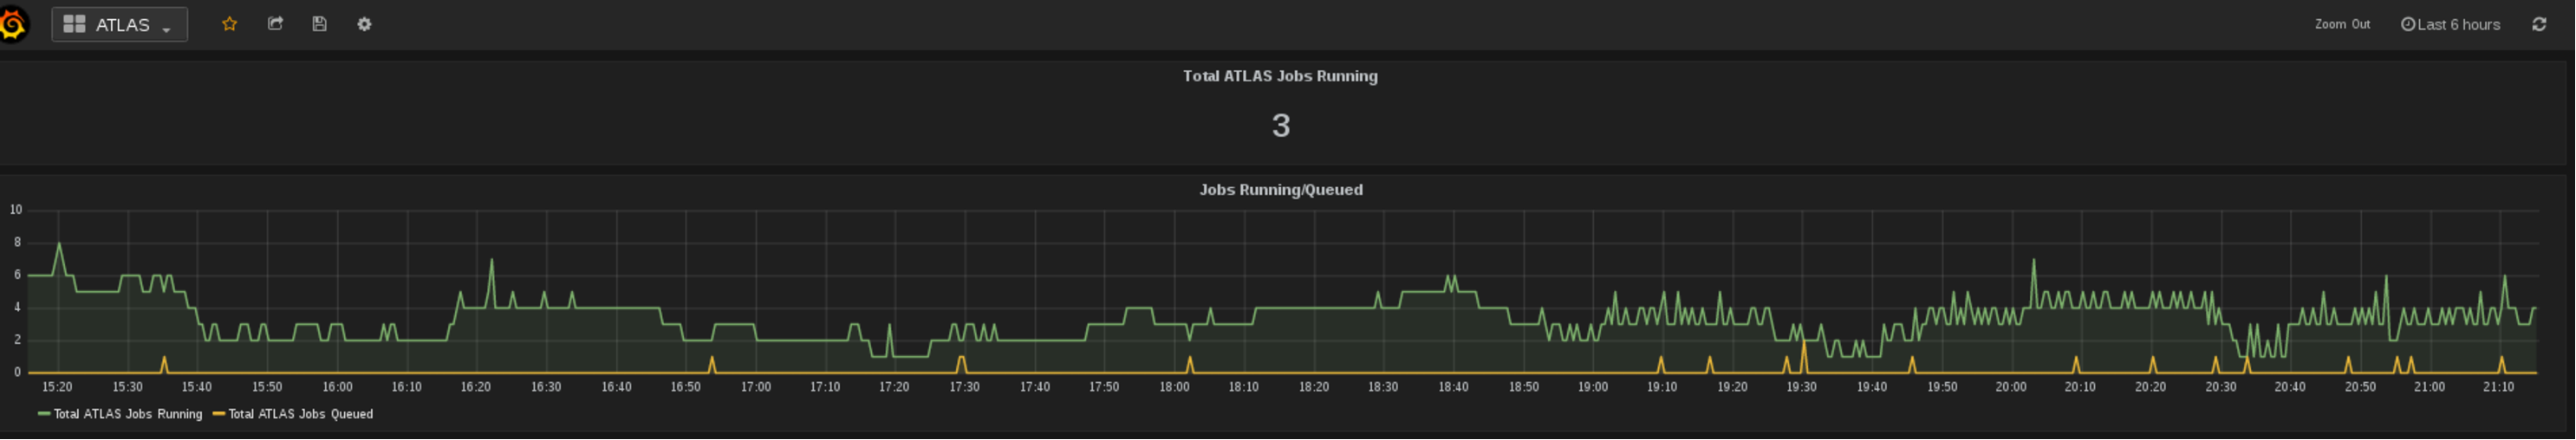
\includegraphics[scale=0.25]{ATLASProcessing-Grafana.pdf}\\
  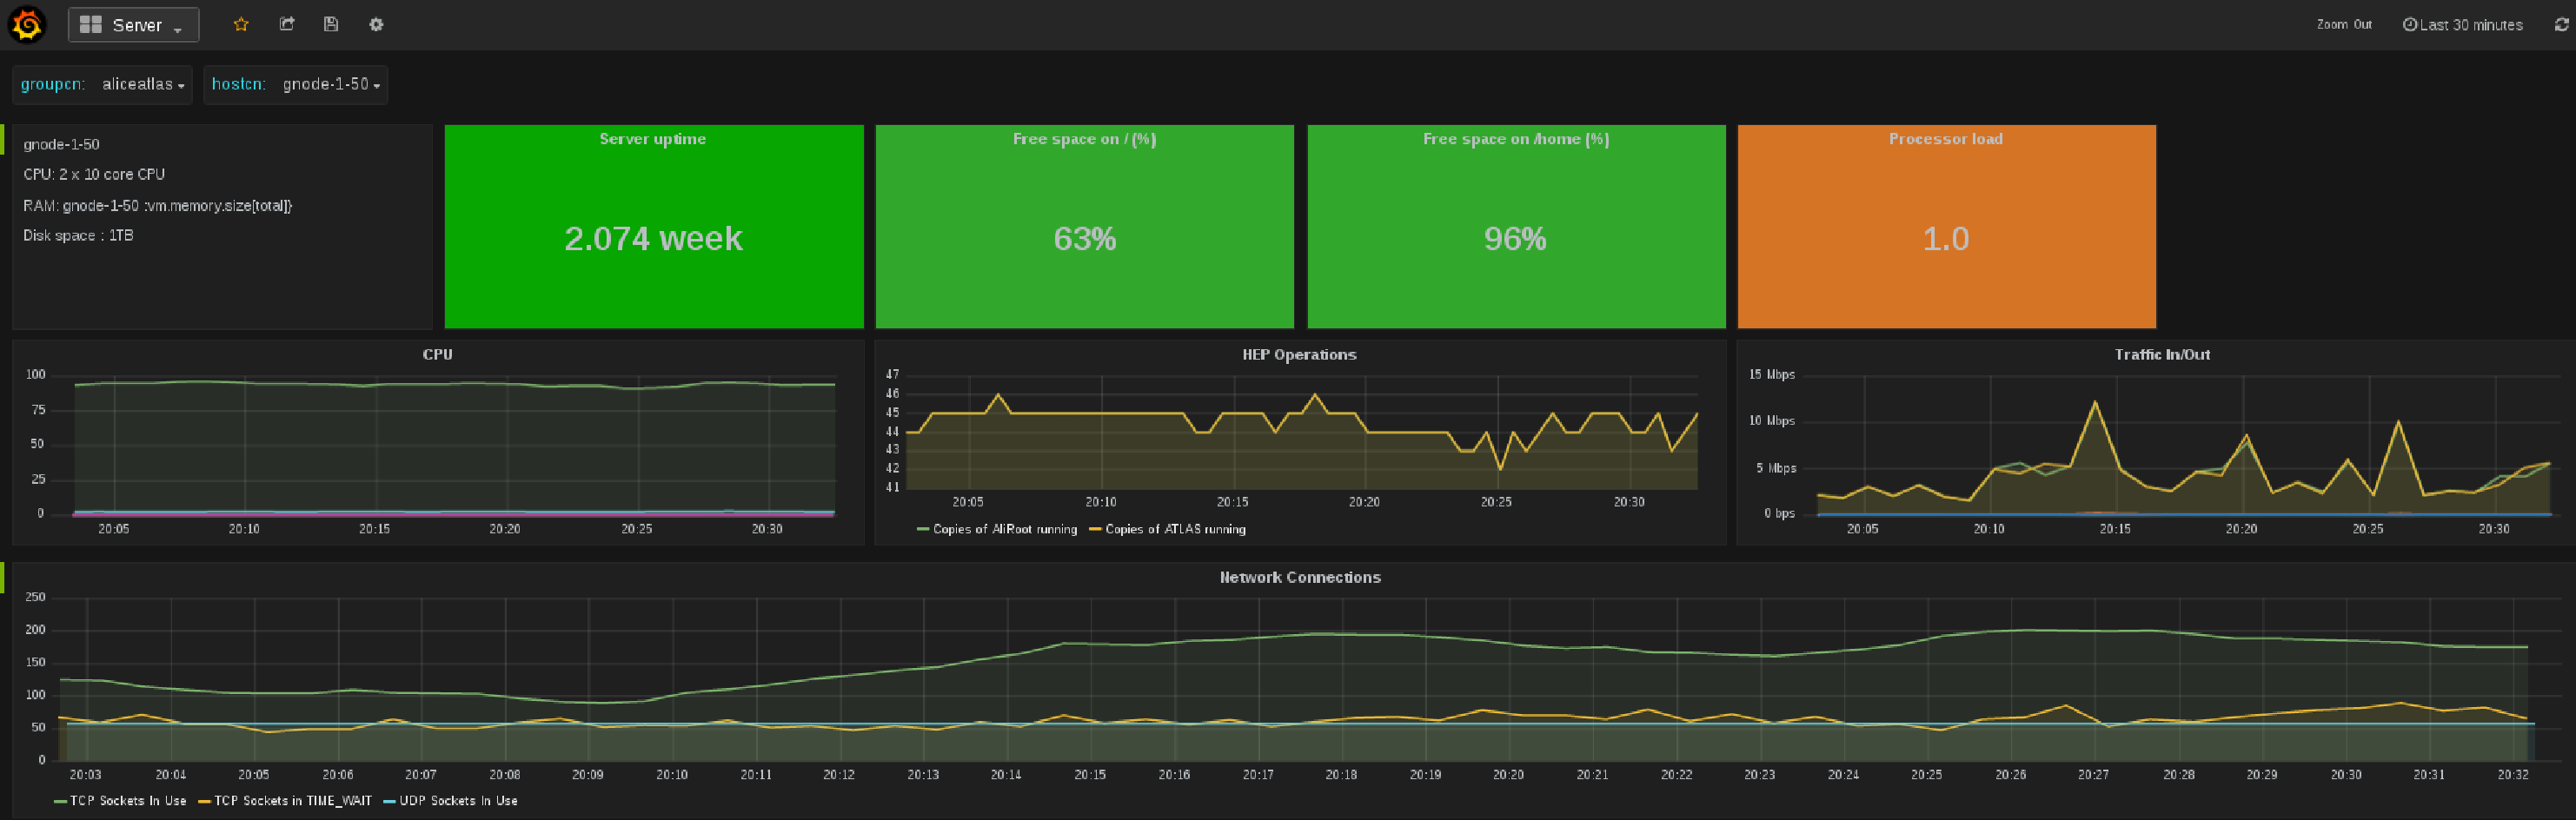
\includegraphics[scale=0.25]{Server50-Grafana.pdf}\\
  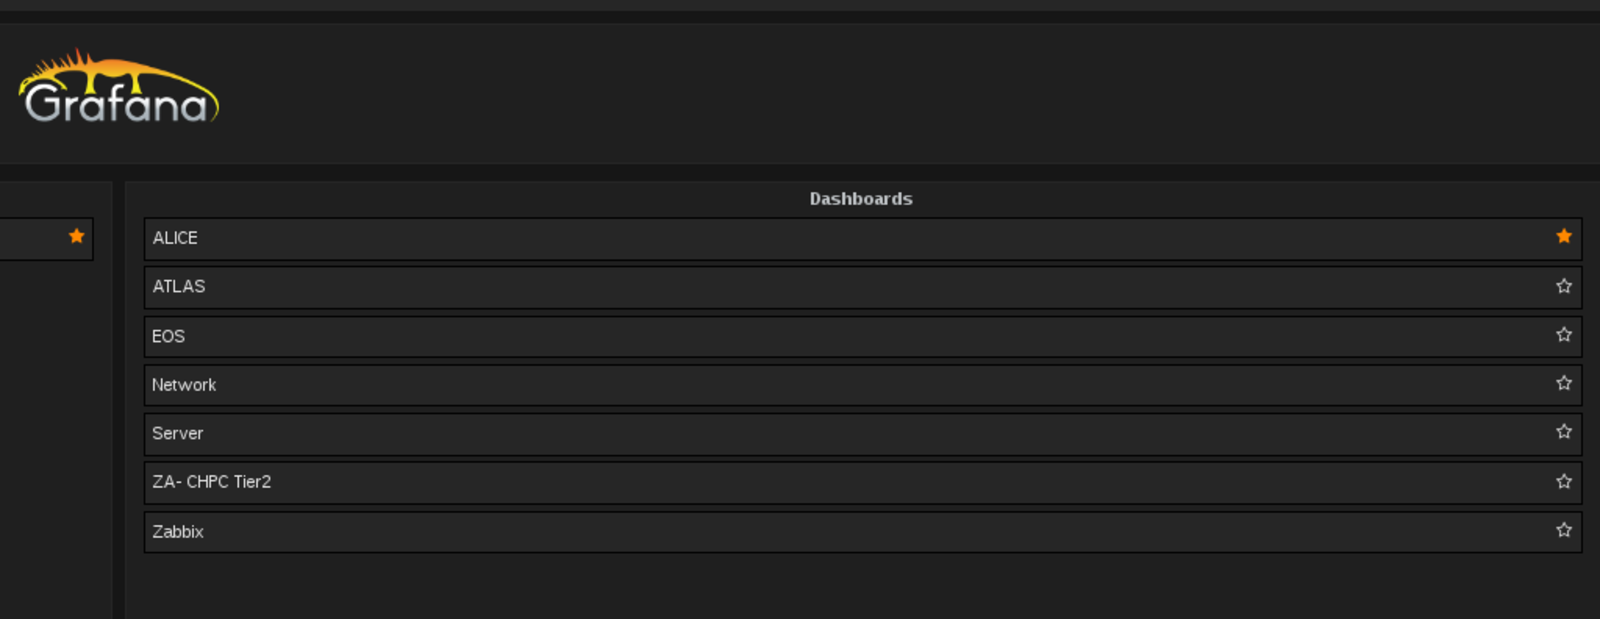
\includegraphics[scale=0.25]{GrafanaMenu.pdf}
\end{frame}


\section{SAGrid, user analysis}
\begin{frame}
\frametitle{28 nodes}
I got the go ahead 3 weeks ago to claim 28 of the 34 nodes back for sagrid and HEP user analysis.
\begin{itemize}
  \item Go back to sagrid to support anybody on sagrid VO.
  \item hep user analysis, based on federated identities, no user account admin.
  \item code based on CODE-RADE, or LHC experiments.
  \item Local Storage for users, eos and lustre.
\end{itemize}
\end{frame}


\begin{frame}
\frametitle{AAROC and SAGrid}
\begin{itemize}
  \item A collaboration spanning Africa and Arabia.\\
  \item Eveything is on github under AAROC.\\
  \item Share the resources of a massively disparate collection of computing resources transparently to the user.\\
  \item Idea of a automated site, via sound deployment tools, and constant integration.
\end{itemize}
\end{frame}

\section{Tier1}

\begin{frame}
\frametitle{Tier 1 Technical Requirements} 
Its a long list but first and foremost :\\
\begin{quote}
  \centering{
  \visible<2->{  \huge{A STABLE, RELIABLE Tier2}}}\\
\end{quote}
\visible<2->{The criticality of that can not be under estimated.}
\end{frame}

\begin{frame}
\frametitle{Tier 1 Technical Requirements} 
\begin{itemize}
  \item Custodial storage of raw data.
  \item O(10k) cores
  \item single digit petabytes storage
  \item redundant links on LHCOPN (light paths to cern) 10Gbps.
\end{itemize}
This is the easy part its just a question of money.\\
The human and process requirements are more onnerous.
\end{frame}

\begin{frame}
  \frametitle{Tier 1 SLA}
  \begin{itemize}
    \item 99\% uptime with beam on.
    \item 4 hour response to failures or degraded service.
    \item  
  \end{itemize}
\end{frame}

\begin{frame}
\frametitle{People Requirements} 
24x7 operation.
storage, hpc, support.
operators on call.
wlcg membership
meetings, meetings, meetings.
\end{frame}
\section{Backup Slides}
\begin{frame}
  \frametitle{LHCOPN}
  \centering{
  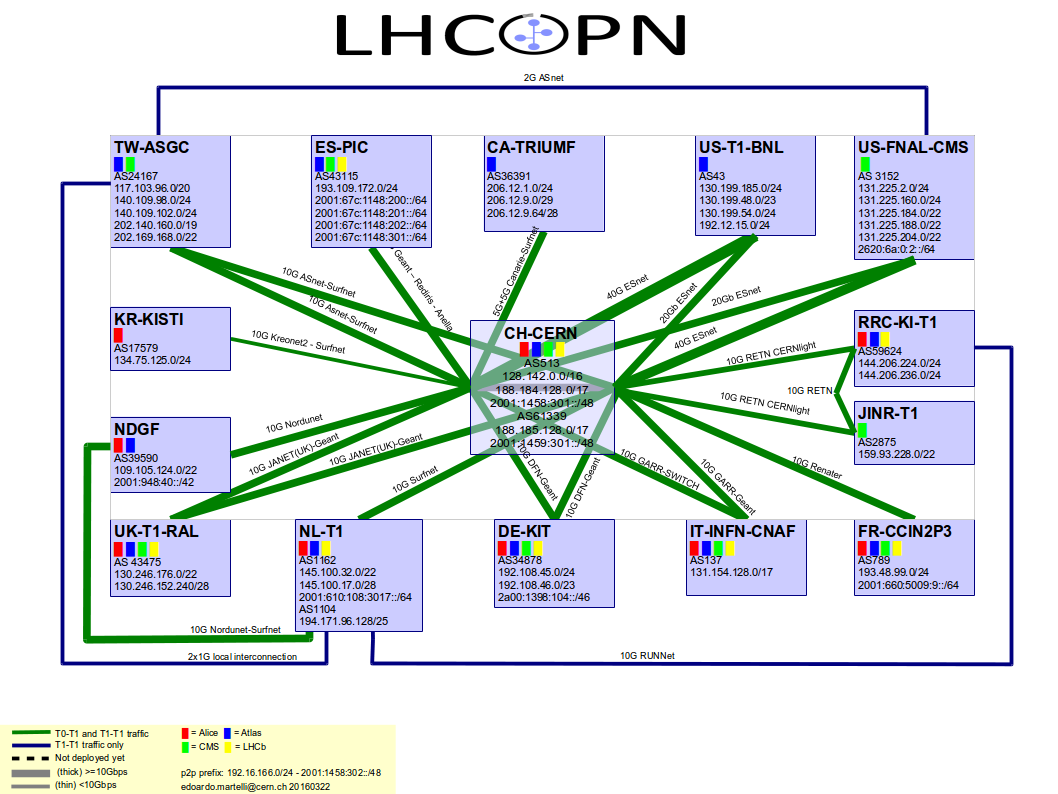
\includegraphics[scale=0.4]{map-lhcopn.png}
  }
\end{frame}

\end{document}
(
